% Latex generates professionally typeset documents. It's different
% from word processors like Microsoft Word in that it separates style from
% content. It lets you write content without worrying too much about things like
% fonts, positioning of tables, and references. Latex has carefully considered
% rules to that sort of that heavy-lifting.

% Latex files are text files where most of the content is the words, sentences,
% and paragraphs. When complete, latex files are fed into the pdflatex program
% to create a pdf - we usually call this compiling the document.

% Within the text you can put comments and commands. These lines are comments.
% On any line, everything after a percent sign (%) is treated as a comment.
% Comments don't have any effect on the output file.

% Commands start with a backslash. The first command is usually \documentclass,
% as below. It tells latex the type of document to generate: book, article,
% letter, etc. Commands can take parameters and/or options.

% Parameters appear in curly braces after the command. Options appear in square
% brackets between the command and the parameters. The \documentclass command
% below has "article" as a parameter and "a4paper" as one option. Multiple
% options are separated by commas.

% Some commands come in pairs like \begin{center} and \end{center}, which is
% usually called an environment. Content in a center environment is centered.

% Latex is built on a language called TeX. TeX is a simple language with only a
% few built-in commands. TeX allows us to create our own commands. LaTeX is a
% huge collection of such programmer-created commands in one handy package.

% There are only a few types of document built-in to latex, like article.
% If you google "latex article options" you'll find lots of sites listing
% what each option does.
\documentclass[a4paper, oneside, hidelinks]{article}

% Lot's of latex programmers have created extra packages for Latex.
% They're not enabled by default as they affect the length of time it takes
% to compile the document. They can enable things like colour and hyperlinks
% in the output pdf. The \usepackage command will include a package, so long
% as it is installed along with latex. TeXLive include lots of standard
% packages by default. Google "latex minted" to see what it does.

% Enables the use of colour. 
\usepackage{xcolor}
% Syntax high-lighting for code. Requires Python's pygments.
\usepackage{minted}
% Enables the use of umlauts and other accents.
\usepackage[utf8]{inputenc}
% Diagrams.
\usepackage{tikz}
% Settings for captions, such as sideways captions.
\usepackage{caption}
% Symbols for units, like degrees and ohms.
\usepackage{gensymb}
% Latin modern fonts - better looking than the defaults.
\usepackage{lmodern}
% Allows for columns spanning multiple rows in tables.
\usepackage{multirow}
% Better looking tables, including nicer borders.
\usepackage{booktabs}
% More math symbols.
\usepackage{amssymb}
% More math fonts, like mathbb.
\usepackage{amsfonts}
% More math layouts, equation arrays, etc.
\usepackage{amsmath}
% More theorem environments.
\usepackage{amsthm}
% More column formats for tables.
\usepackage{array}
% Adjust the sizes of box environments.
\usepackage{adjustbox}
% Better looking single quotes in verbatim and minted environments.
\usepackage{upquote}
% Better blank space decisions.
\usepackage{xspace}
% Better looking tikz trees.
\usepackage{forest}
% URLs.
\usepackage{hyperref}
% For plotting.
\usepackage{pgfplots}
% For filler.
\usepackage{lipsum}
% For line spacing
\usepackage{setspace}
% For changing spacing on pages.
\usepackage{geometry}
% For Gantt charts.
\usepackage{pgfgantt}

% The tikz package allows us to create diagrams and plots using latex
% commands. It defines some extra commands, like \usetikzlibrary below.

% Various tikz libraries.
% For drawing mind maps.
\usetikzlibrary{mindmap}
% For adding shadows.
\usetikzlibrary{shadows}
% Extra arrows tips.
\usetikzlibrary{arrows.meta}
% Old arrows.
\usetikzlibrary{arrows}
% Automata.
\usetikzlibrary{automata}
% For more positioning options.
\usetikzlibrary{positioning}
% Creating chains of nodes on a line.
\usetikzlibrary{chains}
% Fitting node to contain set of coordinates.
\usetikzlibrary{fit}
% Extra shapes for drawing.
\usetikzlibrary{shapes}
% For markings on paths.
\usetikzlibrary{decorations.markings}
% For advanced calculations.
\usetikzlibrary{calc}

% No prizes for guessing what the following few commands do.

% GMIT colours.
\definecolor{gmitblue}{RGB}{20,134,225}
\definecolor{gmitred}{RGB}{220,20,60}
\definecolor{gmitgrey}{RGB}{67,67,67}

% Uncomment for one and a half line spacing.
% \onehalfspacing

% Tell minted to use the following colour scheme. 
\usemintedstyle{manni}
% Set some minted options.
\setminted{frame=lines, framesep=2mm, baselinestretch=1.2, linenos}

% The title.
\title{Research proposal: \\ Improving ELIZA using regular expressions}
\author{Ian McLoughlin (ian.mcloughlin@gmit.ie)}
\date{\today}

% Everything above the below \begin{document} command is referred to as the
% preamble. The preamble configures the features and styles of the output.
% The \begin{document} command tells latex we beginning the content of the
% document - the words, sentences, and paragraphs we want to create.

% Begin the document.  
\begin{document}

  % Display the title in the standard way for the document class.
  \maketitle

  % Usually, the first item after the title is an abstact.
  % An abstract gives a short summary of the main contribution of the document.
  \begin{abstract}
    We propose to research and develop an impovement to Joseph Weisenbaum's
    ELIZA program. The ELIZA program simulates a psychiatrist's questions and
    responses to a patient. The user of the program is the patient in the
    simulation. The program was designed to demonstrate some of the
    superficiality of human conversation. The original program used
    reflective text-based substitutions. Carefully crafted user inputs
    easily demonstrate that they were talking to a simulation rather than a
    person. We are proposing to use regular expressions to further enhance the
    program, making it somewhat more difficult to demonstrate it is a
    simulation.
  \end{abstract}

  % We generally organise our document then in sections. A section is the
  % highest level of organisation, then subsection, then subsubsection. The
  % second subsection of the third section would be listed as part 3.2 of the
  % document. You can either use the command \section{My section} to begin a 
  % new section or you can use \begin{section}{My section} and \end{section} to
  % the same effect. The former is generally preferred as it's cleaner and latex
  % can generally figure out where the section ends.
  \section{Introduction}
    The introduction generally overlaps with the abstract, but expands
    on the ideas. Here, I would discuss the overall proposal and put a context
    around it.
    
    You can start a new paragraph by leaving a blank line. This is a new
    paragraph.
    The introduction should also give a short overview of the rest of the
    document -- a one or two sentence overview of each part of the document.

  % Second section.
  \section{Literature}
    It's important to refer to the existing literature in your proposal. In a
    research proposal I would expect to see at least three or four references
    directly related to the proposal. The next sentence includes a reference.
    % References can be inserted using the \cite{} command with the item's
    % bibtex name in the curly braces. This will insert the reference indicator
    % where the \cite command is called and also ensure the reference title,
    % authours, etc in the list of references. The ~ controls the amount of
    % whitespace around the reference, try googling "latex reference tilde".
    ELIZA is a program written by Joseph Wiesenbaum. It was proposed in his 1966
    paper~\cite{weisenbaumeliza}.
    Wiesenbaum also wrote a book~\cite{weisenbaumcomputerpower}.
    He passed away in 2008~\cite{weisenbaumnytobituary}.
    % We can give most high-level items a label with the \label command.
    % We'll come back to that in a minute.
    \label{section:literature}
    Typically a research proposal will give a bit of background, listing four or
    five directly relevant peer-reviewed publications.

  % Another section.
  \section{Research question}
    All research starts out with an idea. There are no shortage of interesting 
    ideas. An idea needs to be developed into a research question to have a
    reasonable chance of leading to a successful thesis submission.
    
    A research question has a few essential characteristics. It should be clear 
    and specific. It should be informed by the research work of others, as
    described in peer reviewed publications, books, and other reliable sources.
    It should lend itself to an investigation of some sort, that either provides
    evidence as to its answer or answers it outright. The investigation needs to
    be reasonable to complete in the timeframe of the proposed research project.

    It can be difficult to formulate a research question that meets all of those
    characteristics. Research by its nature is tentative. It may seem impossible
    to know ahead of time whether a given investigation could be completed in a
    given timeframe.
    
    The purpose of a research proposal, however, is to demonstrate an
    understanding of the what will be involved in carrying out your research
    project. You will, in consultation with your supervisors, be able to adapt
    your research topic, research question, deliverables, and milestones as the
    project evolves.

    Everything is geared towards helping you to succeed in submitting a
    successful thesis.


  % Another section.
  \section{Timeline}
    This project will take two years to complete. The Gantt chart in Figure
    \ref{figure:ganttchart} gives an overview of the timeline.

    
    \begin{figure}[H]
      \begin{center}
        \begin{ganttchart}[title/.style={draw=none},
                           vgrid, hgrid,
                           canvas/.append style={draw=gmitgrey},
                           bar/.append style={fill=gmitgrey!60}]{1}{24}
          \gantttitle{Q4'20}{3}
          \gantttitle{Q1'21}{3}
          \gantttitle{Q2'21}{3}
          \gantttitle{Q3'21}{3}
          \gantttitle{Q4'21}{3}
          \gantttitle{Q1'22}{3}
          \gantttitle{Q2'22}{3}
          \gantttitle{Q3'22}{3} \\
          \ganttbar{Literature}{1}{3} \\
          \ganttbar{Develop}{4}{12} \\
          \ganttbar{Test}{13}{15} \\
          \ganttbar{Finalise}{16}{24}
        \end{ganttchart}
      \end{center}
      \caption{Gantt Chart}
      \label{figure:ganttchart}
    \end{figure}


  % Let's create a subsection.
  \subsection{Milestones}
    The project will be delivered through a series of milstones. The milestones
    will have the follow deliverables.
    % Here's a description list. Bulleted and numbered lists are similar.
    \begin{description}
      \item[Literature review:] this will be delivered at the end of month 3.
      \item[Chatbot:] this will be delivered at the end of month 12.
      \item[Tests:] the tests will be completed at the end of month 15.
      \item[Thesis:] the thesis will be delivered at the end of month 24.
    \end{description}

  \section{More}
    Latex is great at rendering math.
    $$ math^{works} $$

    \begin{figure}[H]
      \begin{center}
        
\includegraphics[width=200px]{img/gmit-logo.jpg}
      \end{center}
      \caption{The GMIT logo.}
      \label{img:logo}
    \end{figure}
    
    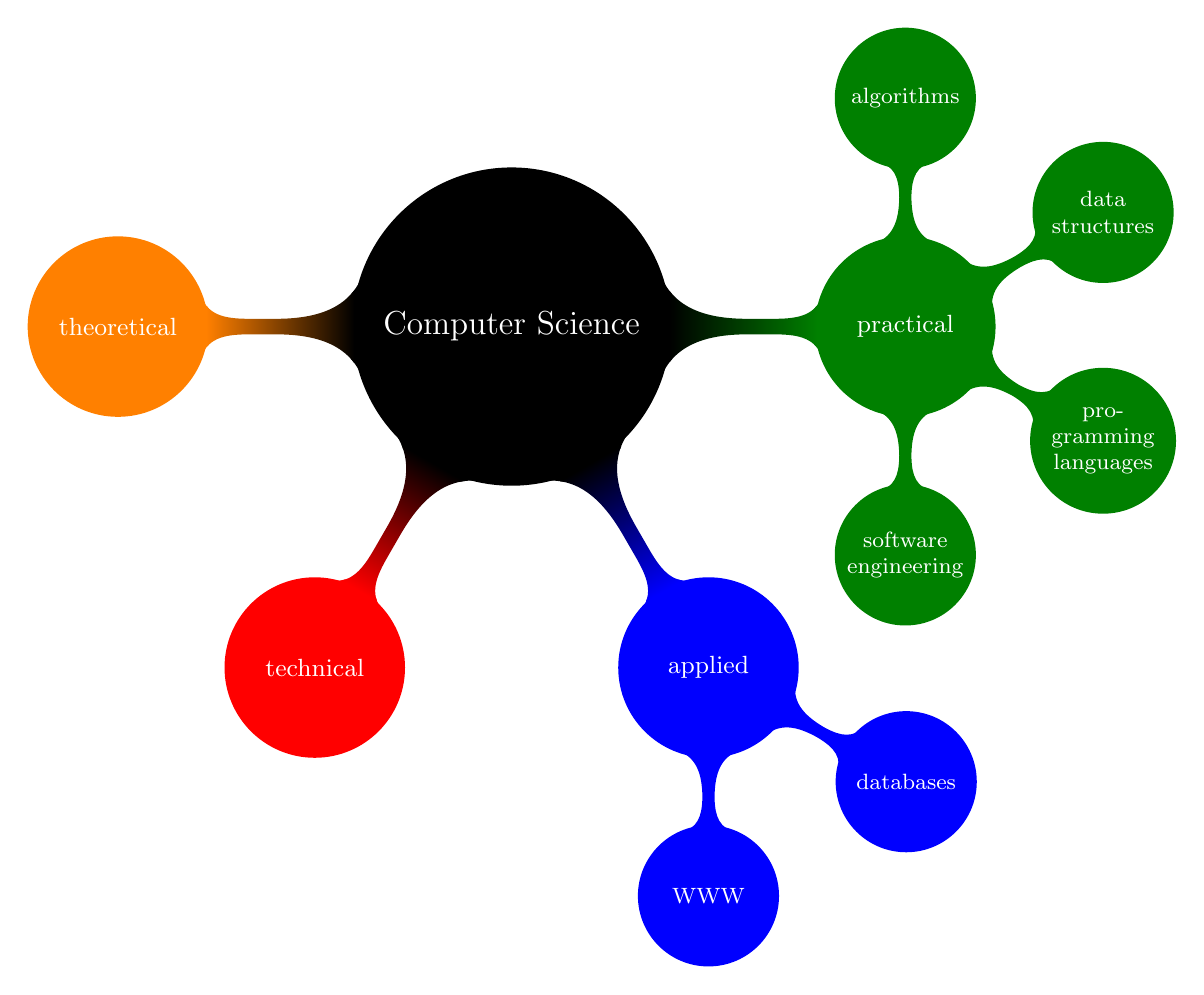
\begin{tikzpicture}
      \path[mindmap,concept color=black,text=white]
        node[concept] {Computer Science}
        [clockwise from=0]
        child[concept color=green!50!black] {
          node[concept] {practical}
          [clockwise from=90]
          child { node[concept] {algorithms} }
          child { node[concept] {data structures} }
          child { node[concept] {pro\-gramming languages} }
          child { node[concept] {software engineer\-ing} }
        }  
        child[concept color=blue] {
          node[concept] {applied}
          [clockwise from=-30]
          child { node[concept] {databases} }
          child { node[concept] {WWW} }
        }
        child[concept color=red] { node[concept] {technical} }
        child[concept color=orange] { node[concept] {theoretical} };
    \end{tikzpicture}

    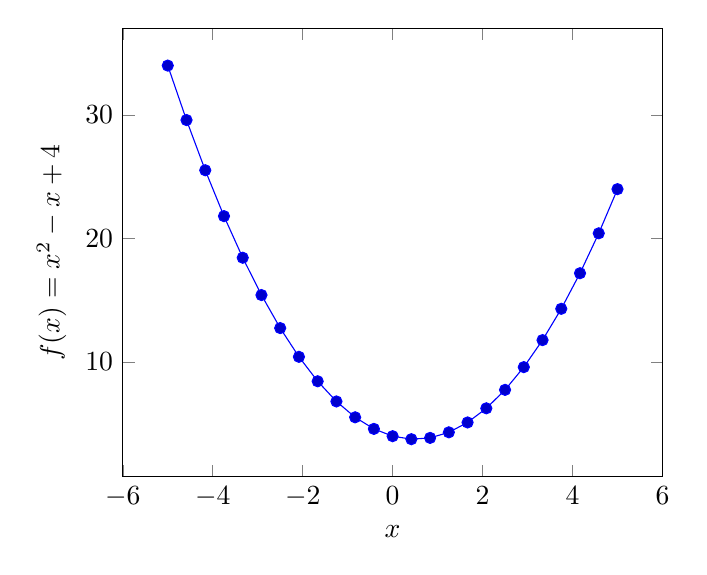
\begin{tikzpicture}
      \begin{axis}[
        xlabel=$x$,
        ylabel={$f(x) = x^2 - x +4$}
      ]
      % use TeX as calculator:
      \addplot {x^2 - x +4};
      \end{axis}
    \end{tikzpicture}
  % Latex together with bibtex will generate a list of references from the
  % \cite commands in the latex document and the items in the bib file.

  % The style of referencing is controlled by the \bibliographystyle command.
  % There are loads of styles available - google "bibtex styles".
  % The ieeetr style uses numbers for references which is common in computing.
  \bibliographystyle{ieeetr}
  % The \bibliography command tells latex where the bib file is. The bib file
  % is called "bibliography.bib" in the current folder. You omit the ".bib".
  \bibliography{bibliography}

% The end of the document.
\end{document}
